% !TEX program = XeLaTeX
% !TEX encoding = UTF-8
\documentclass{article}
 
\usepackage{xeCJK}
\setCJKmainfont{AozoraMinchoRegular.ttf}
\setCJKsansfont{KodomoRounded-Light.otf}
\setCJKmonofont{KodomoRounded-Light.otf}

\usepackage{url}
\usepackage{cancel}
\usepackage{xspace}
\usepackage{graphicx}
\usepackage{multicol}
\usepackage{multirow}
\usepackage{subfig}
\usepackage{amsmath}
\usepackage{amssymb}
\usepackage[a4paper, width=186mm, top=18mm, bottom=18mm, includeheadfoot]{geometry}
%\usepackage[a4paper, width=140mm, top=18mm, bottom=22mm, includeheadfoot]{geometry}
\usepackage{booktabs}
\usepackage{array}
\usepackage{verbatim}
\usepackage{caption}
\usepackage{natbib}
\usepackage{booktabs}
\usepackage{float}
\usepackage{pdflscape}
\usepackage{mathtools}
\usepackage[usenames, dvipsnames]{xcolor}
\usepackage{afterpage}
\usepackage{pgf}
\usepackage{tikz}
\usepackage{dirtree}
\usepackage[style=american]{csquotes}
\usepackage{amsfonts}
\usepackage{tikz}
\usepackage{tkz-graph}
\usetikzlibrary{arrows,decorations.pathmorphing,automata,positioning,backgrounds,fit,shapes.symbols,chains,intersections}

\newtheorem{definition}{Definition}[section]
\newtheorem{theorem}{Theorem}[section]
\newtheorem{lemma}{Lemma}
\newtheorem{proof}{Proof} [section]



\usepackage[toc, page, title, titletoc, header]{appendix}
\usepackage{marginnote}
\usepackage{tablefootnote}

\renewcommand\appendixname{付\ 録}
\renewcommand\appendixpagename{付\ 録}
\renewcommand\appendixtocname{付\ 録}
\renewcommand\abstractname{要\ 約}


\usepackage{perpage} %the perpage package
\MakePerPage{footnote} %the perpage package command

\usetikzlibrary{shapes.geometric}%
\usepackage{color}
%\usepackage[pages=some, placement=top]{background}
\usepackage{eso-pic}
\usepackage[final]{pdfpages}

%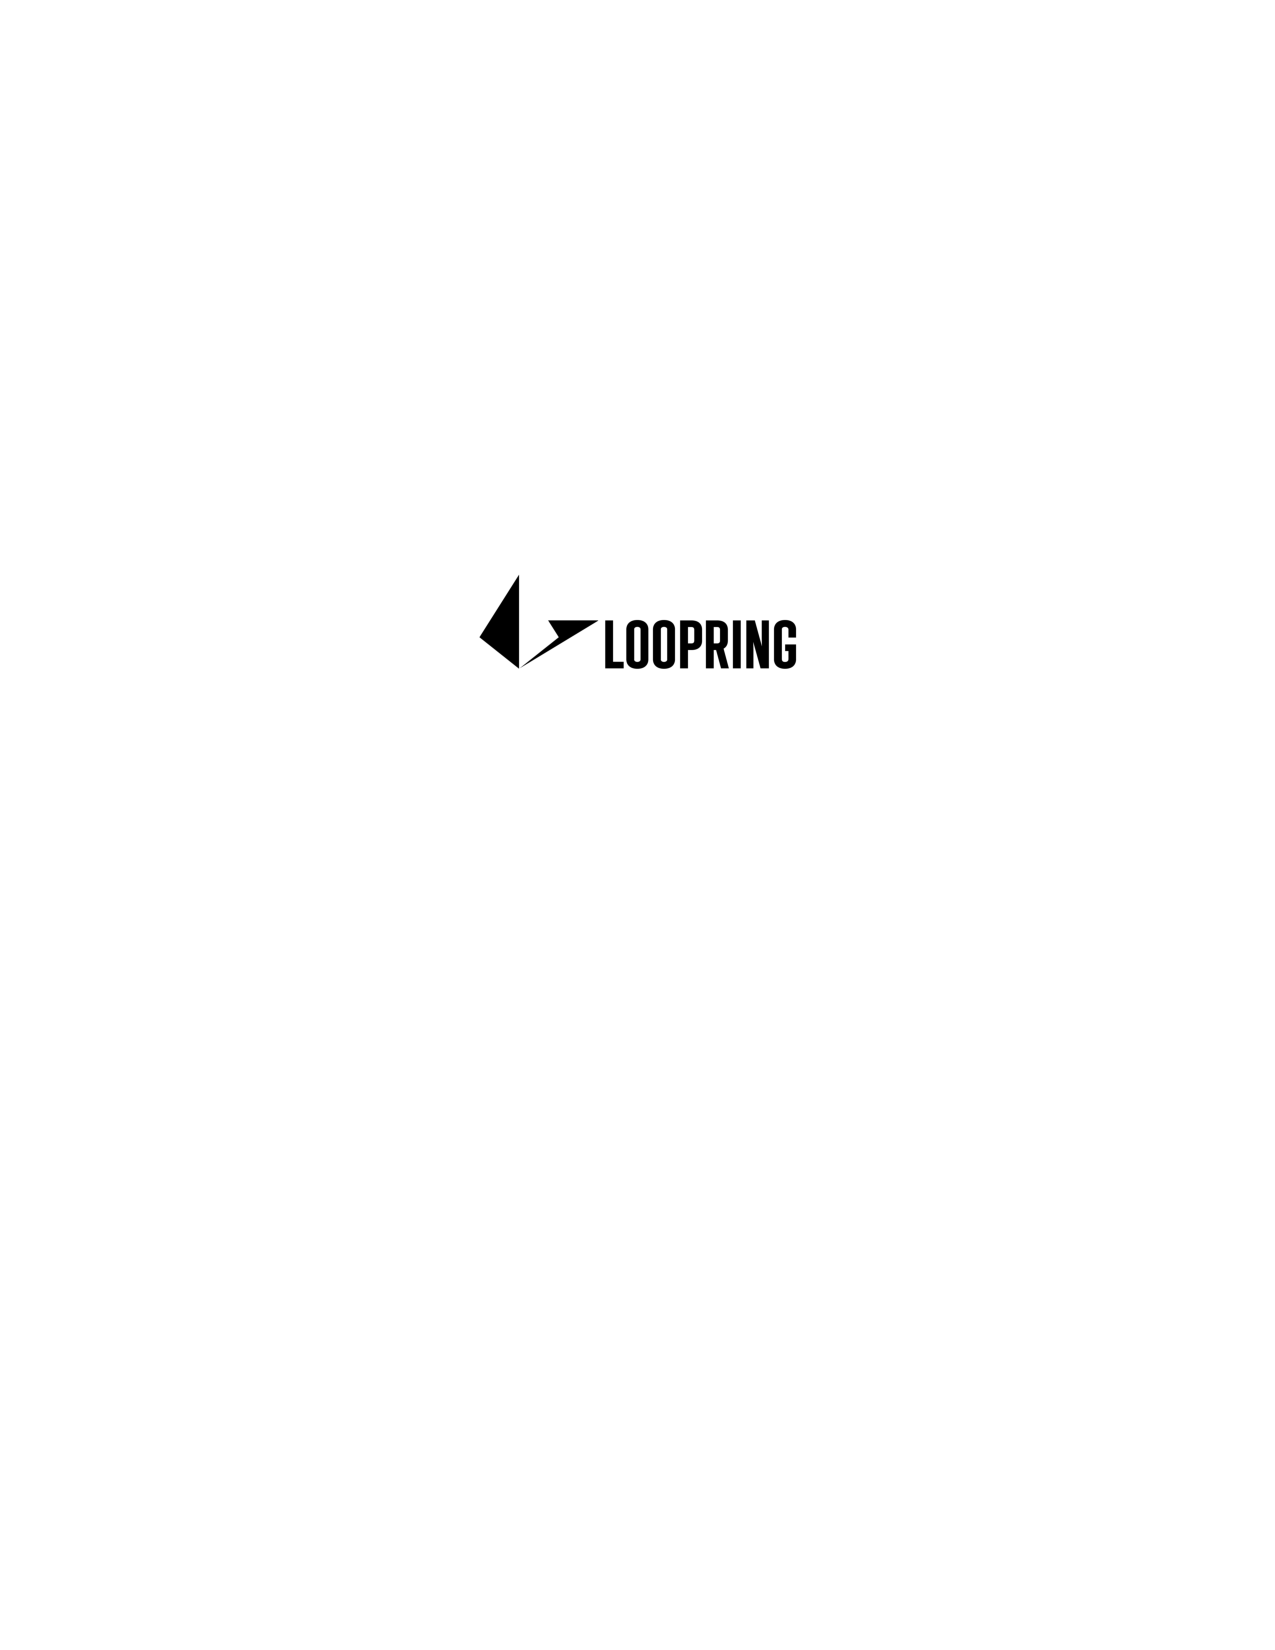
\includepdf[pages=1]{cover}
\hyphenpenalty=750

\title{
{ループリング(LOOPRING):}\\\textbf{分散型トークン取引場プロトコル}}
\author{
  Daniel Wang\\
  \texttt{daniel@loopring.org}\\
  \and
  	Jay Zhou\\
  	\texttt{jay@loopring.org}\\
  	\and
  	Alex Wang\\
  	\texttt{alex@loopring.org}\\
  	\and
  	Matthew Finestone\\
  	\texttt{matt.finestone@gmail.com}\\ 
  \\
  \texttt{https://loopring.org}
 }

\makeatletter
\def\CTEX@section@format{\Large\bfseries}
\makeatother

\makeatletter
\newenvironment{tablehere}
 {\def\@captype{table}}
 {}

\newenvironment{figurehere}
 {\def\@captype{figure}}
 {}
\makeatother
%
%\newcommand\BackgroundPic{%
%\put(0, 0){%
%\parbox[b][\paperheight]{\paperwidth}{%
%\vfill
%\centering
%\includegraphics[width=\paperwidth, height=\paperheight, %
%%keepaspectratio]{images/background.jpg}%
%]{images/background.jpg}%
%\vfill
%}}}


%\begin{document}
%\AddToShipoutPicture{\BackgroundPic}
%\maketitle

\begin{document}
%\AddToShipoutPicture{\BackgroundPic}
\maketitle

\begin{abstract}
ループリングは、分散型取引所を構築するためのオープンプロトコルである。ループリングは、取引と決済を執行するための一連のパブリック・スマートコントラクトとして機能する一方、注文のアグリゲーションと通信はオフ・チェーンで行われる。ループリングのプロトコルは自由度と拡張性が高く、取引機能を組み込んだ分散アプリケーション(dApp)の標準構成要素として機能する。その運用互換性基準はトラストレスかつ匿名の取引を容易にする。現存の分散型取引所のプロトコルと比べ、ループリングが大きく改善した点は、複数の注文による組み合わせを可能にし、2種類のトークンからなる取引ペアの制限を取り除き、劇的な流動性の増加をもたらすことである。また、ループリングはユニークかつ堅固なフロントランニング防止ソリューションを採用している。フロントランニングとは、元のソリューションプロバイダに先立ってブロックにトランザクションを提出するといった不正行為である。ループリングはブロックチェーンに依存せず、スマートコントラクト機能を備えた如何なるブロックチェーンにも配置可能である。執筆時点では、すでにイーサリアム \cite{buterin2017ethereum} \cite{wood2014ethereum}とクアンタム(Qtum)\cite{dai2017smart}のブロックチェーンで運用可能であり、NEO \cite{atterlonn2018distributed}の対応について現在構築中である。
\end{abstract}



\begin{multicols}{2}
\section{導入\label{sec:introduction}}
ブロックチェーンに基づくデジタル資産の急増に伴い、カウンターパーティー間の資産交換・取引の需要が急速に拡大している。特に近年において、数千種類の新しい仮想通貨のトークン(トークン化された伝統的な資産も含む)の出現によって、こうした需要がさらなる拡大を見せている。投機的動機のためであれ、手持ちのネイティブ・ユーティリティ・トークンを通してネットワークへのアクセス権を得るためであれ、仮想通貨間の交換・取引を実現する能力は、より大きいエコシステムの基礎となるであろう。確かに、これらの資産には潜在的なエネルギーがあり\cite{desotocapital}、このエネルギーを解放するため(資本のロック解除)には、所有権の確保だけでなく(この点についてブロックチェーンによって永久に保障されている)、これらの資産を自由に移管・変換する能力もまた必要である。

このように、トラストレスなトークン(バリュー)交換・取引は、まさにブロックチェーン技術の切実な使用例である。しかしながら、現在のところ、仮想通貨の愛好者たちはほとんど伝統的な中央集権型取引所でトークンを取引している。ループリングが必要である理由は、「もし信用された第三者によって二重支払いが起きないように保証されなければならないならば」、ピア・ツー・ピアの電子キャッシュの「主な利点が失われてしまう」といったBitcoin\cite{desotocapital}の主張と同様に、信用された中央集権型取引所で取引されなければならないならば、分散型のデジタル資産の主な利点も失われてしまうからである。

哲学的な観点から見ても、中央集権型取引所で分散型のトークンを取引すること自体も理にかなっていない。分散型のプロジェクトが信奉する理念と一致してないからである。中央集権型取引所に他にも様々な現実的なリスクと限界があるが、これについて後述する。分散型取引所(DEXs) \cite{schuh2015bitshares} \cite{bancor} \cite{kyber}はこれらの問題を解決してきており、ブロックチェーン技術の利用によるディスインターミディエーションを通じてセキュリティリスクの軽減に成功した例もすでに多く見られている。しかしながら、DEXの性能が新しい経済圏における重要なインフラになるにつれ、パフォーマンス面においてまだ改善の余地が大きい。ループリングは、独自のdApp非依存型のオープン・プロトコルによって、前述したインフラのためにモジュラー・ツールを提供することを目的としている。


\section{取引場の現状\label{sec:current_exchange_landscape}}

\subsection{中央集権型取引所の不足点}
中央集権型取引所のリスクについて主に3つの点が挙げられる。1)安全性の欠如、2)透明性の欠如、3)流動性の不足。

\textbf{安全性の欠如} は、ユーザーが自分の秘密鍵(資金)の管理権を中央集権型取引所に委ねることに起因する。これによって、ユーザーは悪意のハッカーによる攻撃の犠牲になるリスクに晒されることとなる。このような中央集権型取引所の安全及びハッキングのリスクは周知されているにもかかわらず \cite{coincheckhack}  \cite{mcmillan2014inside} 、これをしばしば、トークン取引を行う代わりに支払わなければならない対価として受け止められている。そこで現在、中央集権型取引所のサーバーはユーザーの資金を管理しているため、ハッカーにとって格好の攻撃対象となっている。また、取引所の開発者もユーザーの資金を管理するにあたり、誠実かつ予想外のミスを犯す可能性がある。要するに、ユーザーは中央集権型取引所に保管されている自分のトークンに対し管理権を有しないのである。

\textbf{透明性が不足}している状況の下で、ユーザーは不誠実な取引所による不正行為の危険に晒されることとなる。とりわけ取引所の運営者の悪意から、ユーザーが中央集権型取引所で自分の資産の代わりに借用証書(IOU)を取引しているといったこともあるうる。トークンがいったん取引所のウォーレットに送金されれば、取引所は当該トークンの管理権を有する代わりにIOUを発行する。これによってすべての取引は実際にはユーザー間のIOU’sである、ということになる。出金する際に、ユーザーは取引所からIOUを自分のトークンに引き換え、引き出したトークンを自分の外部ウォーレットのアドレスに送金する、といったプロセスになる。このような送金・取引・出金のプロセスには透明性が乏しいだけでなく、取引所自体が閉鎖や破産したり、ユーザーのアカウントを凍結したりする恐れがある。また、ユーザーの資産を第三者に貸し出すなどの不正目的に利用する可能性もある。さらに、透明性の不足はユーザーの資産が全部流出するといった事態を招くことはないとしても、過剰の取引手数料、取引ピーク時の注文処理遅延、規制のリスクやフロントランニングなどリスクが依然として存在する

\textbf{流動性の不足}。取引所の運営者から見ると、流動性の分散は新しい取引所の参入を阻害する効果を持つ。これは二つの「勝者独り勝ちシナリオ」を根拠としている。第一に、ユーザーにとって全ての取引を一つの取引所で行うことが望ましいので、最も多い取引ペアを提供する取引所が勝ち残る。第二に、取引ペアの売買差額が小さい方は有利なので、注文が最も集中する取引所が勝ち残る。これによって新参者による初期の流動性確保が困難になり、競争を阻害することとなる。その結果、多くの取引所はユーザーからの苦情や重大なハッキング事件の多発にもかかわらず、依然として高い市場シェアを維持している。さらに、中央集権型取引所の市場シェアが拡大すればするほど、ハッキング攻撃の対象となる可能性も大きくなることも注意すべきである。 

ユーザーの視点から見れば、流動性の分散化はユーザー・エクスペリエンスを著しく低下させる結果を招く。中央集権型取引所においては、ユーザーは取引所が提供する流動性プール、オーダーブック及び対応取引ペアに基づいて取引するしかない。トークン\verb|A| をトークン\verb|B|に交換するにあたり、ユーザーは両方のトークンを同時に対応している取引所か、あるいは別々の取引所で個人情報を開示して登録しなければならない。また、ユーザーはしばしばBTCやETHなどの主要通貨に基づいて初期または中間取引を行うことが必要となるが、この過程で生じた売買差額を負担しなければならない。最後に、取引が重大な遅延なしに執行されるための注文数が確保されていないこともありうる。取引所が大量取引の処理能力を誇示するとしても、その取引高や流動性は虚偽の情報でない保証はない\cite{fakevolume}。

結果として、伝統的な金融システムと同様に流動性の断片化とエコシステムの分裂化をもたらし、取引は少数の中央集権型取引所に集中することとなる。ブロックチェーン技術がもたらすグローバル規模の流動性は、中央集権型取引所で価値を見出せない結果となるのである。


\subsection{分散型取引所の不足点}

分散型取引所と中央集権型取引所との違いの一つは、ユーザーは直接にブロックチェーンで取引することによって自分の秘密鍵(資産)の支配権を維持できることである。分散型取引所は仮想通貨自体のトラストレス技術を利用して、前述した多くの安全リスクを軽減することができる。しかし、パフォーマンスと構造的制限の問題がまだ残っている。

ユーザーは他の流動性プールと基準からカウンターパートを探さなければならないことから、流動性は問題となっている。ほとんどの分散型取引所またはdAppが相互運用の際に統一した基準を採用しなければ、そして注文が広いネットワークで分散・伝播されなければ、流動性の断片化効果はまだ存在する。指値注文の流動性および弾力性(応じられた注文がどれほど早く再生されること)はユーザーの最善な取引戦略に重大な影響を及ぼしうる\cite{limitorderliquidity}。このような基準の不在は流動性の低下を招くだけでなく、安全上の問題を秘めている一連のスマートコントラクトに暴露されることとなる。

さらに、取引はブロックチェーンの上で行われる以上、分散型取引所には拡張可能性や執行(マイニング)の遅延、注文修正のコストなどのブロックチェーンの限界が内在することとなる。結果として、ブロックチェーンの上でコードを執行するとコスト(ガス)が生じるため、複数の注文がキャンセルされた場合に高額なコストが発生することから、ブロックチェーン・オーダーブックの拡張性が特に優れているわけではない。

最後に、ブロックチェーン・オーダーブックは公開されているため、発送された注文が次のブロックにマイニングされ、オーダーブックに記録されるのを待つ過程において、マイナーは注文の発送を見ることができる。この遅延によって、ユーザーはフロントランニングや、価格または約定が逆方向に動くといったリスクに晒されることとなる。


\subsection{ハイブリッド・ソリューション}
上記の理由から、完全にブロックチェーンに基づく分散型取引所は、その限界によって中央集権型取引所に対し競争上不利の立場に立たされた。こうして、オン・チェーンに内在するトラストレスの特性と、中央集権型の取引スピードや注文処理の柔軟性は、同時に享受できないのである。ループリングや 0x \cite{warren20170x} のようなプロトコルはオン・チェーン決済とオフ・チェーン管理を組み合わせたソリューションを提供する。これらのソリューションはオープンなスマートコントラクトを中心に展開するが、同時にオフ・チェーンで複数の関数を実行し、ノードにネットワークのために決定的な役割を果たせるように柔軟性を持たせることによって、分散型取引所の拡張性の限界を克服する。しかしながら、ハイブリッドモデルにも欠点がある \cite{costofdecent}。ループリング・プロトコルは、本ホワイトペーパーにおいてハイブリッド・ソリューションの欠点を補うために有意義な変更を提案する。

\section{ループリング・プロトコル\label{sec:loopring_protocol}}
ループリング自体は分散型取引所ではなく、複数のブロックチェーンの上で分散型取引所を構成するためのモジュラープロトコルである。我々は伝統的な取引所の構成要素を分解し、代わりに一連のパブリック・スマートコントラクトと分散型の参加者を提供する。このネットワークには、ウォレット、中継器、流動性共有コンソーシアム・ブロックチェーン、オーダーブック・ブラウザー、リングマイナーおよび資産のトークン化サービスといった役割がある。それぞれを定義する前に、まずはループリング・オーダーについて理解する必要がある。

\subsection{ループリング・オーダー\label{sec:order_ring}}
ループリング・オーダーは単指向注文モデル「UDOM」\cite{coinport2014udom}と呼ばれるものによって表示される。UDOMは注文をトークン取引リクエストとして表示し、bidsとasksの代わりにamountS/amountB(売却数量/買付数量)で表示する。個々の注文は2種類のトークン間の交換レートに過ぎないため、このプロトコルの強い特徴は、複数の注文を循環取引によってミキシング・マッチングすることができることである。単一の取引ペアの代わりに最大16個の注文を同時に執行することが可能であるため、流動性の劇的な増加をもたらすだけでなく、価格の改善も期待できる。
 

\begin{center}
\begin{figurehere}
\centering
\tikzstyle{block} = [draw, fill=blue!20, rectangle, 
    minimum height=3em, minimum width=6em]
\tikzstyle{sum} = [draw, fill=blue!20, circle, node distance=1cm]
\tikzstyle{input} = [coordinate]
\tikzstyle{output} = [coordinate]
\tikzstyle{pinstyle} = [pin edge={to-,thin,black}]

\begin{tikzpicture}[
    auto, 
    node distance=2cm,
    >=latex',
    font=\normalfont,
    order/.style={
		scale=0.8,
		rectangle,
		rounded corners,
		draw=black, 
		text centered,
%		text width=10cm,
		minimum height=17mm,
		fill=white
	},
	label/.style={
		scale=0.8
	}
  ]
    % We start by placing the blocks

  \node [order] (order2) 
 {%
 \begin{tabular}{l}
  \textbf{注文\#2}\\
  \textbf{オーナー:Y}\\
  \textbf{売却数量:9B}\\
  \textbf{買付数量:12C}
 \end{tabular}
 };
 
  \node [order, below of=order2, xshift=-3.5cm] (order1) 
 {%
 \begin{tabular}{l}
  \textbf{注文\#1}\\
  \textbf{オーナー:X}\\
  \textbf{売却数量:10000A}\\
  \textbf{買付数量:2B}
 \end{tabular}
 };
 
 
  \node [order, below of=order2, xshift=3.5cm] (order3) 
 {%
 \begin{tabular}{l}
  \textbf{注文\#3}\\
  \textbf{オーナー:Z}\\
  \textbf{売却数量:100C}\\
  \textbf{買付数量:160A}
 \end{tabular}
 };
 
 \draw [draw,->] (order1) -- node [label] {\textbf{7898A}} (order3);
 \draw [draw,->] (order2) -| node [label, xshift=-1.8cm] {\textbf{8B}} (order1);
 \draw [draw,->] (order3) |- node [label, xshift=1cm, yshift=0.24cm] {\textbf{98C}} (order2);

\end{tikzpicture}

\caption{3つの注文からなるオーダー・リング}
\label{fig:ring}
\end{figurehere}
\end{center}

上記の図では、3つの注文からなるオーダーリングの例を示している。それぞれの注文の売却トークン (\verb|tokenS|)は、他の注文の買付トークン (\verb|tokenB|)である。それぞれの注文は対となる反対注文が存在しなくても取引することが可能となり、こうして全ての注文を繋ぐループを作り出す。従来の取引ペアによる取引は実質的にオーダーリングの特例となるが、もちろん執行可能である。


\begin{definition}[オーダーリング]$C_{0}$, $C_{1}$, $\cdots$, $C_{n-1}$ は$n$個の異なる種類のトークンとし、 $O_{0\rightarrow 1}$, $\cdots$, $O_{i\rightarrow i\oplus 1}$, $\cdots$, $O_{n-1 \rightarrow 0}$ は$n$個の注文とする。これらの注文は一つのオーダーリングを形成する:
$$O_{0\rightarrow 1} \rightarrow \cdots \rightarrow O_{i\rightarrow i\oplus 1} \rightarrow \cdots \rightarrow O_{n-1\rightarrow 0} \text{, }$$
nはオーダーリングの長さである場合、 $i\oplus 1 \equiv i+1 \mod n$ となる。
\end{definition}

全ての注文において、利用者が指値した初期レート以上のレートで執行されることが可能の場合、オーダーリングは有効となる。オーダーリングの有効性を検証するために、ループリングプロトコル・スマートコントラクトはリングマイナーからオーダーリングを受信するが、同オーダーリングにあるすべての注文の初期交換レートの積が1以上とならなければならない。

アリスとボブはトークン\verb|A|と\verb|B|を取引しようとすると仮定する。アリスは15個のトークン\verb|A| を持っているが、それを4個のトークン\verb|B|に交換したいと思っている。ボブは10個のトークン\verb|B|を持っているが、それを30個のトークン\verb|A|に交換したいと思っている。

この場合、買い手と売り手はそれぞれ誰となるだろうか?それは、どれのトークンを参照基準にするかによる。トークン\verb|A|を参照基準とする場合、アリスは ${15 \over 4} = 3.75$\verb|A| の価格でトークン\verb|B|を買い付けることになり、ボブは ${30 \over 10} = 3.00$\verb|A|の価格でトークン\verb|B|を売却することになる。トークン\verb|B|を参照基準とする場合、アリスは${4\over 15}=0.26666667$\verb|B|の価格でトークン\verb|A|を売却することになり、ボブは${10 \over 30}=0.33333334$\verb|B|の価格でトークン\verb|A|を買い付けることになる。従って、買い手と売り手が誰になるかは任意である。

前者の場合、アリスの買付指値 ($3.75$\verb|A|)はボブの売却指値 ($3.00$\verb|A|)より高いが、後者の場合、ボブの買付指値 ($0.33333334$\verb|B|)はアリスの売却指値 ($0.26666667$\verb|B|)より高い。明らかに、買い手の指値が売り方の指値と同等または上回る場合に約定が可能となる。

\begin{equation}
{{15\over 4} \over {30\over 10}} = {{10\over 30} \over {4\over 15}}={15 \over 4} \cdot {10 \over 30} = 1.25 > 1
\end{equation}
  
よって、ループを構成する$n$個の注文が全部または一部約定するためには、全ての注文の買付交換レートの積が1より大きくなっているかどうかを知る必要がある。1より大きい場合、$n$個の注文はすべて一部または全部約定することとなる\cite{supersymmetry}。

さらに3人目のカウンターパーティであるチャーリーが加わるとする。チャーリーの加入によって、アリスは$x_1$個のトークン\verb|A|を $y_1$ 個のトークン\verb|B|に、ボブは $x_2$個のトークン\verb|B|を$y_2$個のトークン \verb|C|に、チャーリーは $x_3$個のトークン\verb|C|を $y_3$個のトークン\verb|A|に交換したいといった要求が満されると仮定する。そして必要とされるトークンもすべて揃っているとする。この場合、下記の条件を満せば、取引が可能となる:

\begin{equation}
{{x_1 \cdot x_2 \cdot x_3 \over y_1 \cdot y_2 \cdot y_3} \geq 1}
\end{equation}

ループリング・オーダーの詳細について\ref{anatomy} で後述する。



\section{エコシステムの参加者\label{sec:ecosystem}}
下記のエコシステムの参加者は共同で分散型取引所に求められる機能を提供する。

\begin{itemize}

\item \textbf{ウォレット}:一般的なウォレット・サービスまたはインターフェースであり、ユーザーがトークンにアクセスし、また注文をループリングのネットワークに送信するための方法を提供する。ウォレットはリングマイナーと手数料を分担することによって、注文を生成するためのインセンティブが得られる(詳細は \ref{sec:token}を参照)。我々は、将来にはトークン取引は安全性が確保されたユーザー個人のウォレットで行われるようになることを確信しているため、流動性プールをループリング・プロトコルで結びつけることが最重要である。

\item \textbf{流動性共有コンソーシアム・ブロックチェーン/リレーメッシュ}:注文と流動性の共有のためのリレーメッシュ・ネットワークである。ノードがループリングリレー・ソフトウェアを実行する際に、既存のネットワークに参加し、コンソーシアム・ブロックチェーンを介して他の中継器(リレー)と流動性を共有することができる。我々が構築しているコンソーシアム・ブロックチェーンは世界初の実装であり、ほぼリアルタイム(1-2秒ブロック時間)で注文を共有することが可能であるだけでなく、新しいノードがより迅速にダウンロードできるように古い履歴を調節することができる。特に、中継器はこのコンソーシアムに参加する必要がなく、他の中継器と流動性を共有せずに単独で機能することができ、または独自の流動性共有ネットワークを構築・運営することも可能である。

\item \textbf{中継器/リングマイナー}:中継器は、ウォレットまたはリレーメッシュから注文を受信し、公開されたオーダーブックと取引履歴を管理し、そして(任意のオフチェーン媒体を介して)他の中継器および/またはリレーメッシュ・ノードに注文をブロードキャストすることができるノードである。リングマイニングは中継器の特性であり、要請ではない。リングマイニングの計算量が大きく、完全にオフチェーンで行われる。リングマイニング機能を備えた中継器を「リングマイナー」(\enquote{Ring-Miners})と呼ぶが、リングマイナーは異種の注文をつなぎ合わせてオーダーリングを生成する。中継器は、(1) 相互間の通信方法、(2) オーダーブックの作成方式、および (3) オーダーリングのマイニング方法(マイニングアルゴリズム)を自由に決めることができる。

\item \textbf{ループリングプロトコル・スマートコントラクト(LPSC)}:LPSCは、リングマイナーから受信したオーダーリングをチェックし、ユーザーの代わりにトークンをトラストレスで決済・移動し、手数料をもってリングマイナーとウォレットにインセンティブを与え、イベントを発行する一連の公開・自由のスマートコントラクトである。中継器/オーダーブック・ブラウザは、これらのイベントを待ち受け、オーダーブックと取引履歴を最新の状態に維持する。詳細について付録 \ref{app:protocol_ethereum}を参照。

\item \textbf{資産トークン化サービス(ATS)}:ループリングにおいて、直接的に交換できない資産の間の架け橋である。ATSは、信頼できる企業や組織によって運営されている中央集権型のサービスである。ユーザーは資産(現物や法定通貨、または他のブロックチェーン上のトークン)を預託した代わりにトークンを発行されるが、同トークンをもって預託資産と引き換えることができる。ループリングプロトコルは(適切なソリューションが開発されるまで)クロスチェーン取引のプロトコルではないが、ATSはERC20のトークンと物理的な資産および他のブロックチェーン上の資産\cite{ERC20} の間の取引を可能にする。

\end{itemize}


\section{取引プロセス\label{sec:process}}



\begin{enumerate} 


\item \textbf{プロトコルの承認}: 図\ref{fig:process} では、トークンを取引したいユーザー\verb|Y|は、売却数量のトークン\verb|B|(\verb|amountS|)の売却についてLPSCに承認を与える。ユーザーのトークンは承認によってロックされるわけではなく、ユーザーは注文の処理中においてトークンを自由に移動することができる。

\item \textbf{注文の生成}:最新のトークン\verb|B|とトークン\verb|C|間の交換レートとオーダーブック(板情報)は、中継器またはネットワークに接続された他のエージェント(オーダーブックブラウザなど)によって提供される。ユーザー\verb|Y|は、統合されたウォレット・インターフェースを介して、売却数量(\verb|amountS|)と買付数量(\verb|amountB|)等のパラメータを指定し、指値注文を提出する。一定数のLRxをリングマイナーに支払う手数料として注文に追加することができる。支払う手数料が高いほど、注文はリングマイナーによって処理される可能性が高くなることを意味する。注文のハッシュ値はユーザー\verb|Y|の秘密鍵で署名される。

\item \textbf{注文のブロードキャスト}:ウォレットは注文とその署名を1つまたは複数の中継器に送信する。中継器はその公開されたオーダーブックを更新する。このプロトコルは、先着順などといった特定の方法によるオーダーブックの作成を要求しない。その代りに、中継器は独自のオーダーブックを作成する際に、設計に関する決定権を有する。

\item \textbf{流動性の共有}: 中継器は任意の通信媒体を介して他の中継器に注文情報をブロードキャストする。繰り返しになるが、ノード間の交互方法には自由度がある。ネットワークの接続性を一定レベルに保つため、コンソーシアム・ブロックチェーンを使用した組み込み式の流動性共有リレーメッシュが用意されている。前章で述べたように、このリレーメッシュはネットワークの通信速度と協調性を保てるように最適化されている。

\begin{center}
\begin{figurehere}
\centering
\tikzstyle{block} = [draw, fill=blue!20, rectangle, 
    minimum height=3em, minimum width=6em]
\tikzstyle{sum} = [draw, fill=blue!20, circle, node distance=1cm]
\tikzstyle{input} = [coordinate]
\tikzstyle{output} = [coordinate]
\tikzstyle{pinstyle} = [pin edge={to-,thin,black}]

\begin{tikzpicture}[
    auto, 
    scale=0.6,
    node distance=2.5cm,
    >=latex',
    font=\normalfont,
    order/.style={
		rectangle,
		scale=0.6,
		rounded corners,
		draw=black, 
		text centered,
%		text width=5cm,
		minimum height=12mm,
		minimum width=30mm,
		fill=white
	},
	role/.style={
		circle,
		scale=0.6,
		draw=black, 
		text centered,
%		text width=5cm,
		minimum height=12mm,
		minimum width=12mm,
		fill=white
	},
	steps/.style={
		circle,
		scale=0.6,
		draw=black, 
		text centered,
%		text width=5cm,
%		minimum height=12mm,
%		minimum width=12mm,
		fill=black,
		text=white
	},
	account/.style={
		circle,
		scale=0.6,
		draw=black, 
		text centered,
%		text width=5cm,
		minimum height=16mm,
		minimum width=16mm,
		fill=white
	},
	label/.style={
	  scale=0.6
    }
  ]

 
 \node [role] (user1)  {ユーザーX};
 \node [role, below of=user1] (user2)  {ユーザーY};
 \node [role, below of=user2] (user3)  {ユーザーZ};
 \node [role, below of=user3, fill=gray!20] (relay1)  {中継器M};
 \node [role, below of=relay1, fill=gray!20] (relay2)  {中継器N};

 
 \node [order, left of=user1, xshift=-1cm] (order1) 
 {%
 \begin{tabular}{l}
  \textbf{注文 1}\\
  \textbf{オーナー:X}\\
  \textbf{売却数量:10000A}\\
  \textbf{買付数量:2B}
 \end{tabular}
 };
 
 \draw [draw, ->]  (user1) -- (order1) [label]{};
 \draw [bend right,->] (order1) to node [auto, scale=0.7] {} (relay1);
 \draw [bend right,->] (order1) to node [auto, scale=0.7] {} (relay2);
% \draw [draw, ->]  (order1) |- (relay1) [label]{};
% \draw [draw, ->]  (order1) |- (relay2) [label]{};
 
 \node [order,left of=user2, xshift=-1.5cm] (order2) 
 {%
 \begin{tabular}{l}
  \textbf{注文 2}\\
  \textbf{オーナー:Y}\\
  \textbf{売却数量:9B}\\
  \textbf{買付数量:12C}
 \end{tabular}
 };
 \draw [draw, ->]  (user2) -- (order2) [label]{};
 \draw [bend right,->] (order2) to node [auto, scale=0.7] {} (relay1);
 \draw [bend right,->] (order2) to node [auto, scale=0.7] {} (relay2);
% \draw [draw, ->]  (order2) |- (relay1) [label]{};
% \draw [draw, ->]  (order2) |- (relay2) [label]{};
% 
\node [order, left of=user3, xshift=-2cm] (order3) 
 {%
 \begin{tabular}{l}
  \textbf{注文 3}\\
  \textbf{オーナー:Z}\\
  \textbf{売却数量:100C}\\
  \textbf{買付数量:160A}
 \end{tabular}
 };
 \draw [draw, ->]  (user3) -- (order3) [label]{};
 \draw [bend right,->] (order3) to node [auto, scale=0.7] {} (relay1);
 \draw [bend right,->] (order3) to node [auto, scale=0.7] {} (relay2);
% \draw [draw, ->]  (order3) |- (relay1) [label]{};
% \draw [draw, ->]  (order3) |- (relay2) [label]{};
 
% // The Ring
\node [order, 
yshift=-2.75cm,
xshift=-2.75cm,
below of=relay2,
fill=gray!10,
minimum width=4.5cm,
minimum height=7cm] (ring) {};


\node [order, dashed, below of=relay2,yshift=-0.7cm,xshift=-2.5cm] (order11) 
 {%
 \begin{tabular}{l}
  \textbf{注文 1}\\
  \textbf{オーナー:X}\\
  \textbf{売却数量:10000A}\\
  \textbf{買付数量:2B}
 \end{tabular}
 };
 \node [order, dashed,below of=order11,xshift=-0.25cm,yshift=0.7cm] (order21) 
 {%
 \begin{tabular}{l}
  \textbf{注文 2}\\
  \textbf{オーナー:Y}\\
  \textbf{売却数量:9B}\\
  \textbf{買付数量:12C}
 \end{tabular}
 };
\node [order, dashed,below of=order21,xshift=-0.25cm,yshift=0.7cm] (order31) 
 {%
 \begin{tabular}{l}
  \textbf{注文 3}\\
  \textbf{オーナー:Z}\\
  \textbf{売却数量:100C}\\
  \textbf{買付数量:160A}
 \end{tabular}
 };
 
 % // The blockchain
\node [
rectangle,
fill=gray!20, 
right of=user1,
yshift=-5cm,
xshift=0.1cm,
scale=0.7,
minimum width=3.2cm,
minimum height=17cm] (ブロックチェーン) {\parbox[b][15cm]{1.3cm}{ブロックチェーン}};
% blockchain accounts
  \node [account, right of=user1, xshift=1cm] (account1)  {口座X};
  \node [account, right of=user2, xshift=1cm] (account2)  {口座Y};
  \node [account, right of=user3, xshift=1cm] (account3)  {口座Z};
  \node [account, right of=relay1, xshift=1cm] (account4)  {口座M};
  \node [account, right of=relay2, xshift=1cm] (account5)  {口座N};
  \node [account, double, below of=account5, yshift=-1.4cm] (psc)  {LPSC};
  
 \draw [draw, ->]  (user1) -- (account1) [label]{};
 \draw [draw, ->]  (user2) -- (account2) [label]{};
 \draw [draw, ->]  (user3) -- (account3) [label]{};
% \draw [draw, ->]  (relay1) -- (account4) [label]{};
% \draw [draw, ->]  (relay2) -- (account5) [label]{};
 \draw [draw, double, thick]  (relay1) to node [auto, scale=0.6, xshift=0.5cm, yshift=0.3cm] {流動性の共有}  (relay2) [label]{};
% \draw [draw, ->]  (relay1) -- (ring) [label]{};
 \draw [draw, ->]  (relay2) to node [auto, scale=0.6, xshift=-5cm, yshift=0.5cm] {リングマイニング(ring-mining)}  (ring) [label]{};
 \draw [draw, ->]  (ring) to node [auto, scale=0.6, xshift=1.5cm,  yshift=0.5cm] {提出(submitRing)} (psc) [label]{};
 
 \draw [bend left,->] (account1) to node [auto, scale=0.7] {\textbf{7898 A}} (account3);
 \draw [bend left,->] (account2) to node [auto, scale=0.7] {\textbf{8 B}} (account1);
 \draw [bend left,->] (account3) to node [auto, scale=0.7] {\textbf{98 C}} (account2);
 
 \draw [bend left,->, dashed] (account1) to node [auto, scale=0.7] {} (account5);
 \draw [bend left,->, dashed] (account2) to node [auto, scale=0.7] {} (account5);
 \draw [bend left,->, dashed] (account3) to node [auto, scale=0.7, xshift=.5cm] {\textbf{手数料}} (account5);
  
  
% \draw [draw,->] (order1) -- node [label] {\textbf{7898 A}} (order3);
% \draw [draw,->] (order2) -| node [label, xshift=-1.8cm] {\textbf{8 B}} (order1);
% \draw [draw,->] (order3) |- node [label, xshift=1cm, yshift=0.24cm] {\textbf{98 C}} (order2);

\node [steps, right of=user2, xshift=-0.6cm] () {1};
\node [steps, left of=user2, xshift=0.8cm] () {2};
\node [steps, left of=relay2, xshift=0.3cm, yshift=1cm] () {3};
\node [steps, left of=relay1, xshift=3.6cm, yshift=-1.6cm] () {4};
\node [steps, below of=relay2, xshift=0.3cm, yshift=1cm] () {5};
\node [steps, right of=account3, xshift=-0.6cm] (step5) {6};

 \draw [bend right, ->]  (psc) to node [auto, scale=0.7, xshift=0.5cm] {決済} (step5) [label]{};
 
\end{tikzpicture}

\caption{ループリング取引プロセス}
\label{fig:process}
\end{figurehere}
\end{center}


\item \textbf{リングマイニング(注文マッチング)}:リングマイナーは、指定された交換レート以上のレートで注文を他の複数の注文と全部または部分的にマッチングさせることを試みる。このリングマイナーの働きこそが、このプロトコルはどのペアよりも高い流動性を提供できる主な理由である。執行された交換レートはユーザー \verb|Y|が指定したものより高い場合、マージンはオーダーリング内のすべての注文の間で共有される。リングマイナーは報酬として、マージンの一部を請求する(Margin-Split、LRxはユーザーに返還される)かまたは単に手数料としてLRxを受け取るかを選択することになる。

\item \textbf{検証と決済}:オーダーリングはLPSCによって受信される。LPSCはリングマイナーから提供されたデータを検証し、(オーダーリング内の約定成功率およびユーザーウォレット内のトークン残高によって)オーダーリングが全部または部分的に応じられるか否かを確認するために数回にわたってチェックを行う。全てのチェックが問題なく完了した場合、LPSCは自動的にトークンをユーザーに転送すると同時に、リングマイナーとウォレットに手数料を支給する。ユーザー\verb|Y|の残高が不足しているとLPSCが判定した場合、注文の数量は縮小される(スケールダウン)ことになる。スケールダウンは注文の取消と異なる。スケールダウンは十分な資金が特定のアドレスに預託されれば自動的に元の数量にスケールアップされるが、注文の取消は一方的なマニュアル操作であり、復元することができない。

\end{enumerate}





%
%\end{multicols}
%
%\begin{center}
%\begin{figurehere}
%\includegraphics[height=8cm]{images/en_protocol.png}
%\caption{Loopring Trading Process}
%\label{fig: Loopringrotocol}
%\end{figurehere}
%\end{center}
%
%\begin{multicols}{2}


\section{運用上の柔軟性\label{sec:business_model}}
ループリングのオープンスタンダードは参加者による運用にあたって大きな柔軟性を与えていることは、注目に値すべきである。参加者は自由に新しいビジネスモデルを構築し、ユーザーに価値を提供することができ、同時に(自らそう選択した場合に)取引高などの指標でLRxの手数料を得る。エコシステムはモジュール式であり、より多くのアプリケーションの参加をサポートするために作られた。

\subsection{オーダーブック\label{sec:order_book}}
中継器は、ユーザーの注文の表示とマッチングの方法に関し、様々なオーダーブックを設計することができる。我々が実装した最初のオーダーブックは、指値注文が価格のみに基づいて配置されるといったOTCモデルに従ったものである。言い換えれば、注文のタイムスタンプはオーダーブックと関係がない。しかしながら、中継器は、典型的な中央集権型取引所の注文マッチング・エンジンをエミュレートし、各注文はタイムスタンプを尊重すると同時に価格に基づいてランク付けするというようなオーダーブックを設計することも可能である。中継器にこのタイプのオーダーブックを提供する傾向がある場合は、同中継器はウォレットを所有または統合し、ウォレット・オーダーを同中継器のみに送信するようにすることができ、これによって同中継器は時間に基づいて注文をマッチングすることが可能となる。

一方、他の分散型取引所のプロトコルは時々、中継器に一定のリソース(発注するための初期トークン残高)があることを要請するに対し、ループリングの中継器は、トークンの初期残高無しに、マッチする注文を探し当てるだけで取引を成立させることが可能である。

\subsection{流動性の共有\label{sec:liquidity_sharing}}
中継器は、どのように流動性(注文)を共有するのかを自由に設計できる。ループリングのコンソーシアムブロックチェーンはこれを達成するための一つの解決策であり、中継器はエコシステムの中で自由に相互通信することができる。コンソーシアムブロックチェーンに参加することを除き、中継器は自由にネットワークを構築・運営し、独自のルール/インセンティブを定めることができる。また、タイムスタンプ依存型のウォレット実装でも説明したように、中継器は単独で機能することもできる。もちろん、ネットワーク効果の追求において他の中継器と通信することには明らかなメリットがあるが、ビジネスモデルの多様化は、様々な方法で独自の共有方法の設定と手数料の分担を可能にするといったメリットがある。 


\section{プロトコル仕様\label{sec:protocol}}

\subsection{「注文」の詳細\label{anatomy}}
注文とは、ユーザーが意図する取引を表すデータの集まりである。ループリングにおける注文は、UDOM(the Uni-Directional Order Model、単指向性注文モデル)に従うように定義されている。詳細を以下に示す。

\begin{verbatim}
  message Order {
    address protocol;
    address owner;
    address tokenS;
    address tokenB;
    uint256 amountS;
    uint256 amountB;
    unit256 lrcFee
    unit256 validSince; // システム時刻
    unit256 validUntil; // システム時刻
    uint8   marginSplitPercentage;  // [1-100]
    bool    buyNoMoreThanAmountB;
    uint256 walletId;
    // Dual-Authoring address
    // 二重承認アドレス
    address authAddr;
   // v, r, sで署名を構成する
    uint8   v;       
    bytes32 r;
    bytes32 s;
    // 二重承認用秘密鍵、
    // 注文のハッシュ値計算用ではない、
    // よって署名されていない
    string  authKey; 
    uint256 nonce;         
  }
\end{verbatim}

注文の発信元を確実にするため、\verb|authAddr|を除くパラメータのハッシュ値に対してユーザーの秘密鍵で署名する。 \verb|authAddr|パラメータは、ある注文があるオーダーリングの一部であることを証明し、署名するために使用されるものである。また、それにはフロントランニングを防止する役割もある。詳細は \ref{sec:dual_authoring}を参照。署名は、\verb|v|, \verb|r|, \verb|s|の3つの変数で表され、ネットワークを介して注文パラメータとともに送信される。これにより、注文データは永久に不変であることを証明する。注文データについて、変更されることは有り得ないが、プロトコルはアドレスの残高や他の変数に基づいて最新の状態を計算できる。

UDOMには(本来であれば浮動小数点数でなければならない)指値価格の情報は含まれていない。その代りに、 \verb|amountS|/\verb|amountB|(売却数量/買付け数量)という形式で注文価格を表す。これをレート(\verb|rate|)と呼ぶことにし、略して$r$とも示す。レートは浮動小数点数ではなく、符号なし整数で示される。これは、すべての計算の中間結果を符号なし整数として保持し、計算精度を向上させるためである。


\subsubsection{買付数量}
リングマイナーが注文をリング・マッチングするときに、より良いレートで注文が執行される可能性がある。つまり、ユーザーは、注文時に指定した買付数量(\verb|amountB|)よりも多くの\verb|tokenB|を受け取るする可能性がある。しかし、もし\verb|buyNoMoreThanAmountB|のパラメーラ値が\verb|True|として設定されている場合、ループリングプロトコルは、ユーザーが注文で指定した買付数量(\verb|amountB|)以上の\verb|tokenB|を受け取らないように動作する。したがって、UDOM中の \verb|buyNoMoreThantokenB|パラメータは、注文が完全に約定されたとみなされるタイミングを決定する。\verb|buyNoMoreThantokenB|というパラメータは、売却数量(\verb|amountS|)または買付数量(\verb|amountB|)のいずれかに上限を設定するものであり、従来の注文よりも細かい取引意思を表現することができる。


例えば、\verb|amountS| = 10 かつ \verb|amountB| = 2 の場合、レート$r$ = 10/2 = 5 となる。これはつまり、ユーザーは、1つの \verb|tokenB|につき5つの\verb|tokenS|で交換したい意志を持っていることを示す。もしも、リングマイナーがこの注文に対して、レートが4の反対注文を探り当て、マッチングが成功した場合、ユーザーは、2つではなく、2.5の \verb|tokenB|を受け取ることになる。しかし、ユーザーは、2つの\verb|tokenB|だけ受け取りたく、 \verb|buyNoMoreThanAmountB|のパラメーター値を\verb|True|に設定した場合、LPSCは、1つの \verb|tokenB|を入手するのに4つの\verb|tokenS|を売り出すトランザクションを実行する。その結果、ユーザーにとっては、2つの\verb|tokenS|を節約できたことになる。注意していただきたいのは、説明をシンプルにするために、上記ではマイニング手数料(詳細は \ref{sec:fee_model} を参照)を無視している。

注文の内容を下記の簡易な形式で表現することもできる。

\begin{verbatim}
	      Order(amountS,tokenS,
	            amountB,tokenB,
	            buyNoMoreThantokenB)
\end{verbatim}

例えば、従来の取引場におけるETH/USDのペア市場では、下記の1と3を表現できるが、残りの2と4を表現できない。

\begin{enumerate}
	\item 10 ETHを300USD/ETHのレートで売却することは: \verb|Order(10, ETH, 3000, USD, False)|で表現する。
	\item ETHを300USD/ETHのレートで売却し3000USDを入手することは: \verb|Order(10, ETH, 3000, USD, True)|で表現する。
	\item 10 ETHを300USD/ETHのレートで買付することは: \verb|Order(3000, USD, 10, ETH, True)|で表現する。
	\item 3000USDで10ETH以上でなるべく多くのETHを購入することは: \verb|Order(3000, USD, 10, ETH, False)|で表現する。
\end{enumerate}



\subsection{リング検証\label{sec:ring_verification}}
ループリングのスマートコントラクトは交換レートや売買数量の計算を行わないが、リングマイナーからこれらの値に対する検証結果を受信し、確認する必要がある。これらの計算はリングマイナーによって行われる主な理由は下記の2つである。(1) イーサリアムにおけるsolidity\cite{dannen2017introducing}のようなスマートコントラクト用のプログラミング言語は小数点計算に対応していない。特に $pow(x, 1/n)$ (小数のn次累乗のルートを求める計算)。(2) ブロックチェーンの計算コストを削減するために、計算処理はオフチェーンで行うほうが望ましい。

\subsubsection{サブリング・チェック\label{sec:sub_ring_check}}
このステップは、オーダーリングの中で新しい注文を追加、執行することによって、全てのマージンを独り占めするような不公平なアービトラージ取引を防ぐ。本質的に、有効なオーダーリングがリングマイナーによって見つけられると、オーダーリングに新しい注文を追加すれば、ユーザーにとってのマージン(レート割引)を完全に吸収してしまうことができる。下記の図\ref{fig:subring}に示すように、巧みに計算された$x1$, $y1$, $x2$, $y2$は、すべての注文レートの積を正確に1にするので、ユーザーにとってのレート割引は完全になくなる。

\begin{center}
\begin{figurehere}
\centering
\tikzstyle{block} = [draw, fill=blue!20, rectangle, 
    minimum height=3em, minimum width=6em]
\tikzstyle{sum} = [draw, fill=blue!20, circle, node distance=1cm]
\tikzstyle{input} = [coordinate]
\tikzstyle{output} = [coordinate]
\tikzstyle{pinstyle} = [pin edge={to-,thin,black}]

\begin{tikzpicture}[
    auto, 
    node distance=2cm,
    >=latex',
    font=\normalfont,
    order/.style={
		scale=0.8,
		rectangle,
		rounded corners,
		draw=black, 
		text centered,
%		text width=5cm,
		minimum height=12mm,
		fill=white
	},
	label/.style={
		scale=0.7
	}
  ]
    % We start by placing the blocks

  \node [order] (order2) 
 {%
 \begin{tabular}{l}
  \textbf{注文 2}\\
  \textbf{オーナー:Y}\\
  \textbf{売却数量:9B}\\
  \textbf{買付数量:12C}
 \end{tabular}
 };
 
  \node [order, below of=order2, xshift=-3.5cm] (order1) 
 {%
 \begin{tabular}{l}
  \textbf{注文 1}\\
  \textbf{オーナー:X}\\
  \textbf{売却数量:10000A}\\
  \textbf{買付数量:2B}
 \end{tabular}
 };
 
 
  \node [order, below of=order2, xshift=3.5cm] (order3) 
 {%
 \begin{tabular}{l}
  \textbf{注文 3}\\
  \textbf{オーナー:Z}\\
  \textbf{売却数量:100C}\\
  \textbf{買付数量:160A}
 \end{tabular}
 };
 
   \node [order, below of=order3, yshift=-1cm, fill=gray!20] (order4) 
 {%
 \begin{tabular}{l}
  \textbf{注文 4}\\
  \textbf{オーナー:M}\\
  \textbf{売却数量: x1 A}\\
  \textbf{買付数量: y1 B}
 \end{tabular}
 };
 
 
  \node [order, below of=order1, yshift=-1cm, fill=gray!20] (order5) 
 {%
 \begin{tabular}{l}
  \textbf{注文 5}\\
  \textbf{オーナー: addressM}\\
  \textbf{売却数量: x2 C}\\
  \textbf{買付数量: y2 A}
 \end{tabular}
 };
 
 \draw [draw,->] (order1) -- node [label, xshift=-2cm] {} (order5);
 \draw [draw,->] (order2) -| node [label, xshift=-1.6cm] {} (order1);
 \draw [draw,->] (order3) |- node [label, xshift=1cm] {} (order2);
 \draw [draw,->] (order4) -- node [label, xshift=1.8cm] {} (order3);
 \draw [draw,->] (order5) -- node [label, yshift=0.2cm] {} (order4);
  
\end{tikzpicture}

\caption{サブリングを含むオーダーリングの例}
\label{fig:subring}
\end{figurehere}
\end{center}

ネットワークにゼロバリューを追加することはゼロリスクであるが、これはリングマナーによる不正行為としてみなされる。これを防ぐために、ループリングにおいては、有効なオーダーリングにサブリングを含めることは許されていない。これを確認するために、LPSCは同じトークンが買付注文または売却注文で2回登場しているか否かのチェックを行っている。例えば、上の図では、トークン\verb|A| が2回登場しており、チェックの結果としてこれは不正行為であり、許されないことになる。

\subsubsection{約定率の計算\label{sec:fill_rate_check}}

オーダーリングにおけるレートの計算は、上述の理由により、リングマイナーによって行われる。マイナーによって計算されたレートの正しさをチェックするのはLPSCである。まず、リングマイナーが各注文に対して執行できる買付レートが、ユーザーが設定した元の買付レート以下であることを確認する。これにより、少なくともユーザーが注文時に設定したレートと等しい、或いはより得するレートで、取引が執行されることを保証する。取引レートが確定されると、LPSCはオーダーリング内の各注文が同じ割引されたレートを共有するようにする。たとえば、割引されたレートが$\gamma$である場合、各注文の価格は次のようになる:

$r_{0\rightarrow 1} \cdot (1-\gamma)$, $r_{1\rightarrow 2} \cdot (1-\gamma)$, $r_{2 \rightarrow 0} \cdot (1-\gamma)$, かつ、以下を満たす: 
\begin{equation}
r_{0\rightarrow 1} \cdot (1-\gamma)\cdot r_{1\rightarrow 2} \cdot (1-\gamma) \cdot r_{2 \rightarrow 0} \cdot (1-\gamma) = 1
\end{equation}
したがって: 
\begin{equation}
\gamma = 1- \frac{1}{\sqrt[3]{r_{0\rightarrow 1} \cdot r_{1\rightarrow 2} \cdot r_{2\rightarrow 0}}}\text{.}
\end{equation}
もしトランザクションに$n$個の注文を含んでいる場合、\texttt{割引されたレート}は:
\begin{equation}
\gamma = 1- \frac{1}{\sqrt[n]{\prod_{i=0}^{n-1} r^i}} \text{,}
\end{equation}

ここでは、$r^i$は$i$個目の注文の回転率である。明らかに、ディスカウントレート(discount rate)が $\gamma \ge 0$のときのみ、これらの注文が約定されることができる。そして、$i$個目の注文($O^i$)の実際のレートは: $\hat{r^i} = r^i \cdot (1-\gamma)$, $\hat{r^i}\le r^i$ となる。

前述の例を振り返てみると、アリスは15つのトークン\verb|A|を所有しており、これらを4つのトークン\verb|B|に交換したいと思っている。ボブは10のトークン\verb|B|を所有しており、これらを30のトークン \verb|A|と交換したいと思っている。トークン\verb|A|を基準に考えると、アリスは $\frac{15}{4}$ = 3.75\verb|A| の価格でトークン\verb|B|を買付しようとしている。一方で、ボブは$\frac{30}{10}$ = 3.00\verb|A|の価格でトークン\verb|B|を売却しようとしている。割引(ディスカウント)は: $\frac{150}{120}$ = 1.25 よって、 $\frac{1}{1.25}$ = 0.8 = $(1 −- \gamma)^2$。したがって、この取引において、両者にとって公平なレートは:$\sqrt{0.8}$ $\cdot$ 3.75 $\approx$ 3.3541 トークン\verb|A|/トークン\verb|B| である。

ボブは4つのトークン \verb|B|を渡し、13.4164のトークン\verb|A|を受け取るため、ボブが予期していた12よりも多くトークン\verb|A|を受け取る。一方で、アリスは4つの\verb|B|を受け取るのに13.4164のトークン\verb|A|のみを渡す。これはアリスが予期していた15よりも少なくトークン\verb|A|を渡すことになる。

注意していただきたいのは、一部のマージンはインセンティブとしてマイナー(ウォレット)に渡すことになる。(詳細は \ref{sec:fee_model} を参照)。


\subsubsection{約定状況のトラッキングと注文の取消}

ユーザーは、既に提出した注文の詳細や、キャンセルしたい数量等の情報を含んだ特殊なトランザクションをLPSCに送信することによって、既に提出した注文の全部または一部を取消することができる。
LPSCはこれを考慮に入れ、キャンセルする数量を保管し、\verb|OrderCancelled|というイベントをネットワークに送信する。LPSCは、注文のハッシュ値を注文のIDとして使用することで、該当する注文を特定し、執行された数量と取消された数量をトラッキングし続ける。これらのデータは公開されており、また、 \verb|OrderCancelled| / \verb|OrderFilled|  のイベントはこれらのデータが変更するたびにネットワークに送信される。オーダーリング決済のステップでは、これらの値をトラッキングすることは、LPSCにとってクリティカルなことである。

LPSCはまた、\verb|OrdersCancelled|というイベントで、特定の取引ペアの注文を取消することができ、\verb|AllOrdersCancelled|というイベントで、特定のアドレス中の全ての注文を取消することができる。


\subsubsection{注文の縮小(スケーリング)\label{sec:order_scaling}}
注文は、執行された数量、取消された数量、注文送信者の口座中の現在残高によって、スケーリングされる。この特性に従い、このプロセスはすべての注文のなかで最小約定数量をもつ注文を探し出し、それを参照として、オーダーリング中のすべての注文のスケーリングを行う。

最小約定数量をもつ注文を探し出せば、全ての注文の約定数量の計算が容易になる。
例えば、$i$個目の注文が最小約定数量をもつ注文だとすれば、それぞれの注文で約定される売却数量$\hat{s}$と、それぞれの注文で約定される買付数量$\hat{b}$は、以下のように計算できる:

\[
\begin{split}
&\hat{s}^{i}=\overline{s}_i\text{, } \hat{b}^{i}=\hat{s}^{i}/ \hat{r}^i\text{, }\text{;}\\
&\hat{s}^{i\oplus 1}=\hat{b}^i\text{, } \hat{b}^{i\oplus 1}=\hat{s}^{i\oplus 1}/ \hat{r}^{i\oplus 1}\text{;}\\
&\hat{s}^{i\oplus 2}=\hat{b}^{i\oplus 1}\text{, } \hat{b}^{i\oplus 2}=\hat{s}^{i\oplus 2}/ \hat{r}^{i\oplus 2}\text{;}\\
& ...
%\text{.}
\end{split}
\]
そのなかで、 $\overline{s}_i$ とは約定された後の口座残高を指す。

実際の運用のなかで、オーダーリング中の任意の注文が最小約定数量を持つ注文だと仮定し、オーダーリングのなかでループ処理を行って、最大2回の計算を行うだけでそれぞれの注文の約定数量を計算できる。

例えば、最小約定数量が注文の中で指値した数量の5\%である場合、オーダーリング中のすべての注文の約定数量は5\%に縮小(スケールダウン)される。約定後、最小約定数量をもつ注文はすでに全部約定されるはずである。

\subsection{オーダーリング決済\label{sec:settlement}}

オーダーリングが前述のすべてのチェックを通過していれば、そのオーダーリングはクローズドとなり、決済に移ることができる。これは、$n$個の注文はひとつの閉じられたループで繋げられることを意味する。その様子を下記の図に示す。

\begin{center}
\begin{figurehere}
\centering
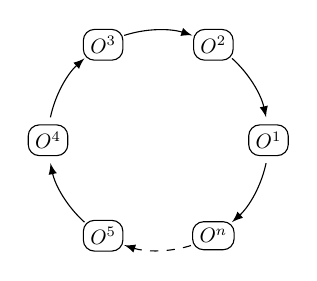
\begin{tikzpicture}[
circle/.style={
		scale=0.75,
		rounded corners,
		draw=black, 
		text centered,
		}
]

\def \n {6}
\def \m {4}
\def \radius {1.4cm}
\def \margin {12} % margin in angles, depends on the radius

\foreach \s in {1,...,\m}
{
  \node[draw, circle] at ({360/\n * (\s - 1)}:\radius) {$O^\s$};
  \draw[<-, >=latex] ({360/\n * (\s - 1)+\margin}:\radius) 
    arc ({360/\n * (\s - 1)+\margin}:{360/\n * (\s)-\margin}:\radius);
}

\node[draw, circle] at ({360/\n * 4}:\radius) {$O^5$};
  \draw[<-, dashed, >=latex] ({360/\n * 4+\margin}:\radius) 
    arc ({360/\n * 4+\margin}:{360/\n * (5)-\margin}:\radius);
    
\node[draw, circle] at ({360/\n * 5}:\radius) {$O^n$};
  \draw[<-, >=latex] ({360/\n * 5+\margin}:\radius) 
    arc ({360/\n * 5+\margin}:{360/\n * (6)-\margin}:\radius);


\end{tikzpicture}
\caption{オーダーリング決済}
\label{fig:settlement}
\end{figurehere}
\end{center}

決済を完了させるのに、\verb|TokenTransferDelegate|(トークン移動/送金用のデリゲート)という名のスマートコントラクトがLPSCによって使用される。このようなデリゲートの導入はスマートコントラクトのアップグレードをより容易にする。なぜなら、注文は、プロトコルのバージョンを考慮する必要がなく、このデリゲートをオーソライズさえすれば良いのである。

オーダーリングのそれぞれの注文について、約定状況により、一定の\verb|tokenS|を前後の注文に支払うことになる。また、マイナーにも選択された手数料モデルに従い手数料をを支払う。最後に、全ての決済が完了すれば、\verb|RingMined|(オーダーリングマイニング完了)といういイベントを生成する。


\subsubsection{イベントの生成\label{sec:events}}

ループリングプロトコルはイベントを生成することにより、オーダーブックの最新状況を、中継器、オーダーブラウザー、及びその他のエコシステム参加者にいち早く知らせる。イベントの種類を以下に示す。

\begin{itemize}
	\item \textbf{OrderCancelled}:特定の注文が取消された際のイベント。
	\item \textbf{OrdersCancelled}:特定のユーザーのアドレス中、一つの取引ペアに関する注文が取消された際のイベント。
	\item \textbf{AllOrdersCancelled}:特定のユーザーのアドレス中、すべての取引ペアに関する注文が取消された際のイベント。
	\item \textbf{RingMined}:特定のオーダーリングの決済が完了した際のイベント。このイベントには、リング中におけるトークン移動履歴データが含まれている。
\end{itemize}


\section{LRx トークン\label{sec:token}}
「LRx」は、ループリングトークンの一般表記である。「LRC」はイーサリアムのブロックチェーン上の、「LRQ」はクアンタム(Qtum)上の、「LRN」はNEO上のトークンである。今後は、LRxが他のパブリックブロックチェーンでトークンが開発されるにつれ、順次に紹介する予定である。

\subsection{手数料モデル\label{sec:fee_model}} 
ユーザーは注文を作成するとき、リングマイナーに支払う手数料として、LRxの数量とリングマイナーが請求できるマージン分担比率 (\verb|marginSplitPercentage|)を指定する。これをマージンスプリットと言う。リングマイナーはLRxとマージンスプリットのどちらを報酬として受け取るかを選択することができる。

以下の図は典型的なマージンスプリットの例を示している:

\begin{center}
\begin{figurehere}
\centering
\begin{tikzpicture}[
scale=1,
font=\normalfont,
classical/.style={thick,<->,shorten >=2pt,shorten <=2pt,>=stealth},
oneway/.style={->,dashed,shorten >=2pt,shorten <=2pt,>=stealth}
]
    % Draw axes
    \draw [->,thick] (0,1) node (yaxis) [above] {$$}
        |- (6.2,0) node (xaxis) [right] {$$};
        
    \draw
  	(4,0) coordinate (A)
  	(4,1) coordinate (A2)
  	(4.8,-0.6) coordinate (B)
  	(4.8,1) coordinate (B2)
  	(6,-0.6) coordinate (C)
  	(6,1) coordinate (C2);
  	
  	\fill [draw=none, fill=gray!20] 
    (4.8, 0) rectangle (6, 1);
    
  	\fill [draw=none, fill=gray!10] 
    (0, -0.6) rectangle (4.8, 0);

	\draw[thick] (0, -0.6) -- (0, 0.6) node[below]{$$};
  	\draw[thick, thin] (A) -- (A2) node[below]{$$};
  	\draw[thick, thin] (B) -- (B2) node[below]{$$};
  	\draw[thick] (C) node[below, xshift=0.5cm]{買付数量合計} -- (C2) ;
  	
  	\draw[classical] (0, 0.5) -> (4, 0.5) node[below]{$$};
  	\draw[classical] (4, 0.75) -> (4.8, 0.75) node[below]{$$};
%  	\draw[classical] (4.8, 0.5) -> (6, 0.5) node[below]{$$};
  	\draw[classical] (4, 0.25) -> (6, 0.25) node[below]{$$};

  	
  	\draw[oneway] (2, 1.2) node[above]{注文指値買付数量} -- (2, 0.5);
  	\draw[oneway] (4.4, 2.2) node[above]{追加買付数量} -- (4.4, 0.75);
  	\draw[oneway] (5.4, 1.6) node[above, xshift=0.4cm]{マージンスプリット} -- (5.4, 1);
  	\draw[oneway] (5, -1.2) node[below]{マージン} -- (5, 0.25);
  	\draw[oneway] (2.4, -1.2) node[below]{注文実質買付数量} -- (2.4, -0.5);



\end{tikzpicture}
\caption{マージンスプリットが60%の場合}
\label{fig:marginsplit}
\end{figurehere}
\end{center}

オーダーリング状のマージンが少なすぎる場合、リングマイナーはLRxを報酬として選択し、反対にマージンが十分に大きく、マージンスプリットがLRxを大きく上回る場合、リングマイナーはマージンスプリットを選択する。但し、リングマイナーがマージンスプリットを選択した場合、ユーザー(発注者)に対して、ユーザーが手数料としてリングマイナーに支払うはずだったLRxの数量と同等なLRxを支払う必要がある。これのことはリングマイナーがマージンスプリットを選択する場合の敷居をLRxを選択した場合の2倍まで高めることとなり、結果としてLRxを報酬として選択する傾向を強化することとなる。よって、リングマイナーはマージンの高いオーダーリングでより少ない収入を得ることのトレードオフとして、マージンの低いオーダーリングで安定的に収入を得ることが可能となる。ループリングの手数料モデルは、マージンの高いオーダーリングが市場の成長・成熟につれ減少することによって、固定のLRx手数料は必然的にインセンティブとして必要されるようになるといった期待に基づいている。

下記の図に示されている状況が予想される。

\begin{center}
\begin{figurehere}
\centering
\begin{tikzpicture}[
font=\normalfont,
oneway/.style={->,dashed,shorten >=2pt,shorten <=2pt,>=stealth},
scale=1]
    % Draw axes
    \draw [<->,thick] (0,2.7) node (yaxis) [above] {$y$}
        |- (5,0) node (xaxis) [right] {$x$};
        
    \draw
  	(1,1) coordinate (A)
  	(2,1) coordinate (B);
  	
  	
  	\draw[thick] (B) -- (3.7,2.7);
  	\draw[dotted] (B) -- (2,0) node[below] {$2f$};
  	\draw[dotted] (A) -- (1,0) node[below] {$f$};
  	\draw[thick,color=gray!70] (0,0) -- (2.7,2.7);
  	\draw[thick] (0,1) node[left] {$f$}--(B) node[     ]{$$};
 	\draw[oneway] (4,1) node[right]{期待されるマイニング収入} -- (3, 2);


\end{tikzpicture}
\caption{ループリングの手数料モデル}
\label{fig:feemodel}
\end{figurehere}
\end{center}

 $f$ をLRx手数料、$x$軸をマージンスプリット、$y$軸をマイニングによる収入とする。$y=max(f, x-f)$ は黒実線で示したとおりであるが、もしLRx手数料=0であれば、$y=max(0, x - 0)$ は灰実線で示している。


結果は以下の通りとなる:
\begin{enumerate}
	\item マージンスプリットが0の場合、リングマイナーはまだインセンティブ効果があるLRx手数料を選択する。
	\item LRx手数料が 0の場合、結果は灰実線となり、収入は一般線形モデルに基づくこととなる。
	\item マージンスプリット収入が2x(LRx手数料)を超える場合、リングマイナーはマージンスプリットを選択して、ユーザーにLRxを支払う。
\end{enumerate}

注意すべきなのは、LRx料金が0でない場合、リングマイナーがどのオプションを選択しても、リングマイナーと発注者の間にLRxの移動が必ず発生する。すなわち、リングマイナーはLRx手数料を獲得するか、またはLRx手数料を発注者に支払い、マージンスプリットを受け取ることとなる。

それと、リングマイナーはウォレットと一定比率の手数料を共有する。ユーザーがウォレットを通して注文を送信し、それが執行されると、ウォレットは一定のLRx手数料またマージンスプリットを報酬として受け取る。こうした設計はモジュール式であり、独自のビジネスモデルまたは実装は可能であるが、我々の慣例はウォレットが手数料の約20\%-25\%を受け取ることである。ウォレットはユーザー基盤があるためループリングプロトコル・インテグレーションの主要ターゲットではあるが、収入源がほとんどないからである。


\subsection{分散型ガバナンス}

メンバー間の協調による効率的な目標達成という意味では、ループリングプロトコルは根本的にソーシャルプロトコルである。この点は、一般の暗号通貨界隈のプロトコルと異なるわけではなく、実際にその有用性は調整問題 \cite{vitalikgovernance}、グリムトリガー均衡、限定合理性等と同様なメカニズムによって保護されている。つまり、LRxトークンは手数料として支払うためのものだけでなく、多数のネットワーク参加者の報酬金を調整するためにも使用される。このような調整機能はどのプロトコルが幅広く採用されるために必要であるが、取引所は分散型エコシステムにおける流動性の向上によって成否が決定されるため、こうした調整機能は取引所のプロトコルにとって特に重要である。

LRxトークンは、分散型ガバナンスを通じてプロトコルの更新のためにも使用される。スマートコントラクトの更新は継続性と安全性を確保し、非互換性による流動性低下のリスクを軽減するためにトークン所有者によって管理される。スマートコントラクトはいったんデプロイされると変更できなくなるため、dAppまたはエンドユーザーが古いバージョンのものと交互し、更新されたコントラクトから除外されるといったリスクが存在する。プロトコルは市場の需要と基盤となるブロックチェーンに適応しなければならないため、アップグレード可能性はプロトコルの成功にとって非常に重要である。LRxのステークホルダーによる分散型ガバナンスの下で、スマートコントラクトはdAppやエンドユーザーを妨害せず、またはスマートコントラクトの抽象化に過度に依頼せずに更新することが可能となる。LRxトークンの発行量は固定である。例えばLRCの場合、一部はループリング財団に帰属し、また一部はコミュニティーに提供するための基金に配分されることとなる。

しかしながら、LRxトークンの所有者はプロトコルの発展方向を決める唯一のステークホルダーではない。ほかには、中継器・リングマイナーや開発者などもエコシステムの不可欠の構成員部であり、彼らの意見も無視してはならない。実際に、これらの構成員はそれぞれの役割を果たすにはLRxの所有が必要とされないことを鑑みると(伝統的な買い手・売り手やマーケットメーカーが存在しないため、初期におけるトークンの保有は強制的ではない)、彼らの利益を確保するために代替的な方法を許可しなければならない。さらに、「単なる」トークンによる投票は、オンチェーン・オフチェーンにかかわらず、低い投票率やトークン所有権の集中はリスクをもたらすため、意見の相違を和らげる方法としては不十分である。従って、我々の目標は、多層からなるガバナンスモデルおよび共有知識に基づく意思決定のプロセスのルールを構築することである。これを達成するために、あらゆる参加者や(可能ならば)予定されたプロトコルのフォーカスポイントからの意見を収集する協調機構から、一定のサポートを得ることが期待できる。この目標が実現すれば、ループリング財団は必然的にプロトコルの開発者役から執事役へと進化するであろう。


\section{詐欺と攻撃に対する防衛措置}

\subsection{フロントランニングの防止\label{sec:dual_authoring}}

分散型取引所におけるフロントランニングとは、別のノードの取引ソリューションをコピーし、保留中のトランザクションプール(メモリプール)にあるコピー元のトランザクションに先だってマイニングすることである。これはより高い取引手数料(ガス価格)を指定することで可能となる。ループリング(または他の注文マッチングプロトコル)において、主なフロントランニング・スキームは「注文の横取り(order-filch)」であり、すなわち、フロントランナーが保留中のオーダーリング決済トランザクションから1つ以上の注文を横取りすることである。また、ループリングにおいて保留中のトランザクションからオーダーリングを丸ごと横取りすることさえありうる。

サブミットリング(submitRing)トランザクションがまだ確認されておらず、未処理のトランザクションプールに残っている場合、誰もが簡単にこのトランザクションを見分け、\verb|minerAddress|を横取り屋である自分のアドレス(\verb|filcherAddress|)に置き換えることができる。次に、\verb|filcherAddress|でペイロードを辞退して、オーダーリングの署名を置き換えることが可能になる。最後に、横取り屋は、より高いガス価格を設定し、新しいトランザクションを提出すると、ブロックマイナーが元のsubmitRingトランザクションの代わりに自分のトランザクションを次のブロックに書き込むのを待てば良いのである。

この問題に対する従来の解決策には重要な欠点がある:より多くの取引が必要となり、その結果より多くのガス費用がかかることと、オーダーリングを決済するのに、少なくとも2倍のブロックの数が必要となることである。我々が提供する新しいソリューションである「二重承認(Dual Authoring)」\cite{dualauthor}には、注文の決済とリングマイニングについてそれぞれ承認を必要とするといった二段階による承認を設定する仕組みを含む。


二重承認のプロセスは下記の通りである。

\begin{enumerate}

	\item ウォレット・ソフトウェアは各注文についてランダムな公開鍵/秘密鍵のペアを生成し、その鍵ペアを注文のJSONスニペットに入れる。(別の方法として、公開鍵の代わりに公開鍵から派生したアドレスを使用してバイト・サイズを減らす方法がある。このようなアドレスを「\verb|authKey|」と表記し、認証アドレスと一致する秘密鍵を「\verb|authAddr|」と表記する。)


	\item \verb|r|, \verb|v|, \verb|s|, 及び \verb|authKey| を除いて、注文にあるすべての項目に基づいてハッシュ値を計算し、そのハッシュ値に対してオーナーの秘密鍵(\verb|authKey|)で署名する。

	\item ウォレットはリングマイニングのために\verb|authKey|とともに注文を中継器に送信する。リングマイナーは、\verb|authKey|と\verb|authAddr|が正しくペアになり、注文の署名がオーナーのアドレスに関して有効であることを検証する。

	\item オーダーリングが識別されると、リングマイナーは各注文の\verb|authKey|を使用して、リングのハッシュ値、 \verb|minerAddress|およびすべてのマイニングパラメータに署名する。オーダーリングに $n$個の注文が含まれている場合、$n$個の\verb|authKey|sによって$n$個の署名が作成される。これらの署名を「\verb|authSignature|s」と言う。また、リングマイナーは\verb|minerAddress|の秘密鍵を使用して、すべてのマイニングパラメータとともにリングのハッシュに署名する必要がある。

	\item リングマイナーは、すべてのパラメータと余分の\verb|authSignature|sでsubmitRing関数を呼び出す。\verb|authSignature|s はオンチェーンのトランザクションの一部ではないため、リングマイナー以外の当事者に知られていないことを注意しよう。

	\item ループリングプロトコルは各注文に対応する\verb|authAddr|に対し、それぞれの\verb|authSignature|を検証するが、 \verb|authSignature|が存在しない或いは無効の場合は拒否される。


\end{enumerate}

結果として:

\begin{itemize}

	\item  各注文の(オーナーアドレスの秘密鍵による)署名は、\verb|authAddr|を含む注文が変更不能であることを保証する。
	\item  リングマイナーの( \verb|minerAddress| の秘密鍵による)は、提供された場合において、誰もそのリングマイナーのIDでオーダーリングをマイニングすることができないことを保証する。
	\item  \verb|authSignature|sは、 \verb|minerAddress|を含むオーダーリング全体が変更不能であることと、注文の横取りが不可能であることを保証する。

\end{itemize}

二重承認は、オーダーリングの決済が1つのトランザクションの中で決済されることを確保すると同時に、「オーダーリング横取り」と「注文横取り」を防止する。それに加えて、二重承認は中継器が2つの方法によって注文を共有することを可能にしている。ノンマッチャブル共有(nonmatchable sharing)とマッチャブル共有(matchable sharing)。デフォルトは、ループリングはOTCをモデルに運営し、指値注文のみに対応するため、注文のタイムスタンプは無視されることとなる。このことは、フロントランニングは対象取引の価格に影響を与えないが、取引が実行されるかどうかに影響を及ぼすことを意味する。

\section{その他の攻撃}

\subsection{シビル攻撃とDOS攻撃}

悪意のあるユーザーは、ループリングノードを攻撃するために大量の小規模な注文を送信する可能性がある。しかし、ほとんどの場合において、ノードはこれらの注文をマッチングしても満足のいく利益を出せないことを理由にこれらの注文を拒否するであろう。中継器は自らどのように注文を取扱うのかを決める権限があるため、脅威として大量な小さな注文による攻撃は発生しない。

\subsection{残高不足}
悪意のあるユーザーは、実際のアドレスでは残高がゼロであるにも関わらず、注文数量がゼロでないことを偽った注文を署名し、送信する可能がある。その際、ノードは、実際の残高がゼロであることを監視して気付くことができる。状況に応じてこれらの注文状態を更新し、破棄することもできる。ノードは、注文のステータスを更新するために時間を費やさなければならないが、たとえば、アドレスをブラックリストに登録し、関連する注文を無効にすることなどもできる。

\section{まとめ}

ループリングプロトコルは、分散型取引所の基盤レイヤーとなることを目指しており。 人々の資産や価値の交換方法を劇的に変えるものである。金銭は、中間財であり、取引の媒体として機能しており、取引の両者が互いの物品あるいはサービスを手に入れたい際の「欲求の二重の一致」(Double Coincidences of Wants)問題 \cite{unenumerated2006}を解決している。それと同様に、ループリングプロトコルは、取引をより簡単に完結させるためにリング・マッチングを使用することによって、取引ペアにおける欲求の二重の一致への依存性を取り除くことを目指している。これは、社会や市場がトークンや伝統的な資産をどのように交換するのかという点で大きな意味を持つ。実際に、分散型の仮想通貨は、国家の金銭に対する支配権を脅かしているのと同じように、トレーダー(消費者/生産者)を結びつけるプロトコルは、金銭の概念自体に対する理論的な脅威である。

ループリングプロトコルには以下のメリットがある。

\begin{itemize}
	\item オフチェーンの注文管理とオンチェーンの決済によってパフォーマンスを低下させることなく、安全性を確保。
	\item リングマイニングと注文の共有による流動性の増大。
	\item 分散型取引場における大きな問題であるフロントランニングをデュアルオーサーリングで徹底的に防止。
	\item スマートコントラクトがオープンで無料であり、あらゆるdAppでプロトコルを使用可能。
	\item オペレータ間の標準化は、ネットワーク効果をもたらし、ユーザーエクスペリエンスを改善。
	\item オーダーブックとコミュニケーティングによるフレキシブルなネットワーク管理
	\item 参入敷居が低く、ノードがネットワーク及びエンドユーザーに参加するコストが低い。
	\item ウォレットによる直接的な匿名取引が可能。
\end{itemize}

\section{謝辞}
本書を作成するにあたり、メンター、アドバイザー、及びコミュニティーの皆様から、ご指導、ご協力をいただいた。ここに深謝の意を表する。特に、本プロジェクトにてレビューとフィードバックをしていただいた白碩(ChinaLedgerより)、闞海濱教授、Alex Cheng、達鴻飛、曹寅、呉暁川、王震、于偉、段念、肖軍、銭江、向江旭、郭一鵬、李大海、Kelvin Long、夏華夏、馬俊、及びEncephalo Pathに感謝の意を表する。


\bibliography{whitepaper}
\bibliographystyle{unsrt}


\end{multicols}


%\begin{appendices}
%
%\section{EVM(Ethereum Virtual Machine)上のループリングプロトコルの実装\label{app:protocol_ethereum}}
%
%\begin{center}
%\begin{figurehere}
%\centering
%\begin{tikzpicture}
%[node distance = 1cm, auto,font=\footnotesize,
%% STYLES
%every node/.style={node distance=3.5cm},
%% The comment style is used to describe the characteristics of each force
%comment/.style={rectangle, inner sep= 7pt, text width=4cm, node distance=0.25cm, font=\scriptsize\sffamily},
%% The force style is used to draw the forces' name
%force/.style={rectangle, draw, fill=black!10, inner sep=5pt, text width=4cm, text badly centered, minimum height=1.2cm, font=\normalfont}] 
%
%% Draw forces
%\node [force] (impl) {LoopringProtocolImpl};
%\node [force, dashed, above of=impl] (protocol_interface) {LoopringProtocol};
%\node [force, left=1cm of impl] (nameregistry) {NameRegistry};
%\node [force, right=1cm of impl] (tokenregistry) {TokenRegistry};
%\node [force, below of=impl] (delegate) {TokenTransferDelegate};
%\node [force, left=1cm of delegate] (multisig) {TransferableMultsig};
%
%%%%%%%%%%%%%%%%
%% Change data from here
%
%% impl
%\node [comment, below=0.25 of impl] (comment-impl) {- オーダーリングの検証\\
%- 決済のためのトークン移動(送金)\\
%- イベントの発行};
%
%% nameregistry
%\node [comment, below=0.25cm of nameregistry]{- ウォレットと中継器の登録};
%
%% protocol_interface
%\node [comment, below=0.25 of protocol_interface](comment-interface) {- インターフェースとイベントの定義};
%
%% tokenregistry
%\node [comment, below=0.25 of tokenregistry] {- ERC20/ERC223 トークンの登録};
%
%% delegate
%\node [comment, below=0.25 of delegate] {- ユーザーの代わりにトークンを移動(送金)};
%
%% PUBLIC POLICIES
%\node [comment, text width=3cm, below=0.25 of multisig] {- マルチシグネチャーオーナーシップの有効化
%};
%
%%%%%%%%%%%%%%%%%
%
%% Draw the links between forces
%\path[->,thick] 
%(comment-interface) edge (impl)
%(nameregistry) edge (impl)
%(tokenregistry) edge (impl)
%(delegate) edge (comment-impl);
%
%\end{tikzpicture} 
%\caption{スマートコントラクト}
%\label{fig:smartcontracts}
%\end{figurehere}
%\end{center}
%
%\section{スマートコントラクトのデプロイメント}
%
%\subsection{Ethereum}
%下記スマートコントラクトは既にイーサリアム(Ethereum)のメインネットにデプロイ済みである:
%\begin{itemize}
%\item LRC: \verb|0xEF68e7C694F40c8202821eDF525dE3782458639f|
%\item TokenRegistry: \verb|0xa21c1f2AE7f721aE77b1204A4f0811c642638da9|
%\item TokenTransferDelegate: \verb|0x7b126ab811f278f288bf1d62d47334351dA20d1d|
%\item NameRegistry: \verb|0xd181c1808e3f010F0F0aABc6Fe1bcE2025DB7Bb7|
%\item LoopringProtocolImpl: \verb|0x0B48b747436f10c846696e889e66425e05CD740f|
%\end{itemize}
%
%\subsection{Qtum}
%下記スマートコントラクトは既にクアンタム(Qtum)のメインネットにデプロイ済みである:
%\begin{itemize}
%\item LRQ: \verb| 2eb2a66afd4e465fb06d8b71f30fb1b93e18788d |
%\item TokenRegistry: \verb| c89ea34360258917daf3655f8bec5550923509b3 |
%\item TokenTransferDelegate: \verb| 60b3fa7f461664e4dafb621a36ac2722cc680f10 |
%\item NameRegistry: \verb| e26a27d92181069b25bc7283e03722f6ce7678bb |
%\item LoopringProtocolImpl: \verb| 5180bb56b696d16635abd8dc235e0ee432abf25d |
%\end{itemize}
%
%\end{appendices}
\end{document}